% Parked 2026-09-13: the USRP/RHS bench frames (IEEE/CIC ICCC 2024 demo) and their
% Stop-5 signpost, removed from the Class 5 lecture. Not part of the build.

% Inserted 2026-09-09. Reprise of the tour map: the USRP bench appeared with no
% connection to the FSO frames before it. The link is the tour itself: four stops
% of theory earn the objection "does any of this exist?", and the bench answers it.
\begin{frame}{Stop 5: out of the simulator}
  \vspace{0.4em}
  \centering
  \tourmap{5}

  \vspace{0.9em}
  {\small\raggedright Four stops of optimisation problems. By now you have earned
   a blunt question: \textbf{does any of this exist outside a paper?}\par}

  \vspace{0.4em}
  {\small\raggedright Last stop: a lab bench where both beams are real --- one
   aimed at a user, one at a target --- and where the measured numbers come out
   \textbf{humbler} than the simulated ones. That gap is the honest part.\par}
\end{frame}

\begin{frame}{Somebody actually built one}
  \vspace{0.3em}
  \begin{columns}[T,onlytextwidth]
    \column{0.42\textwidth}
      \centering
      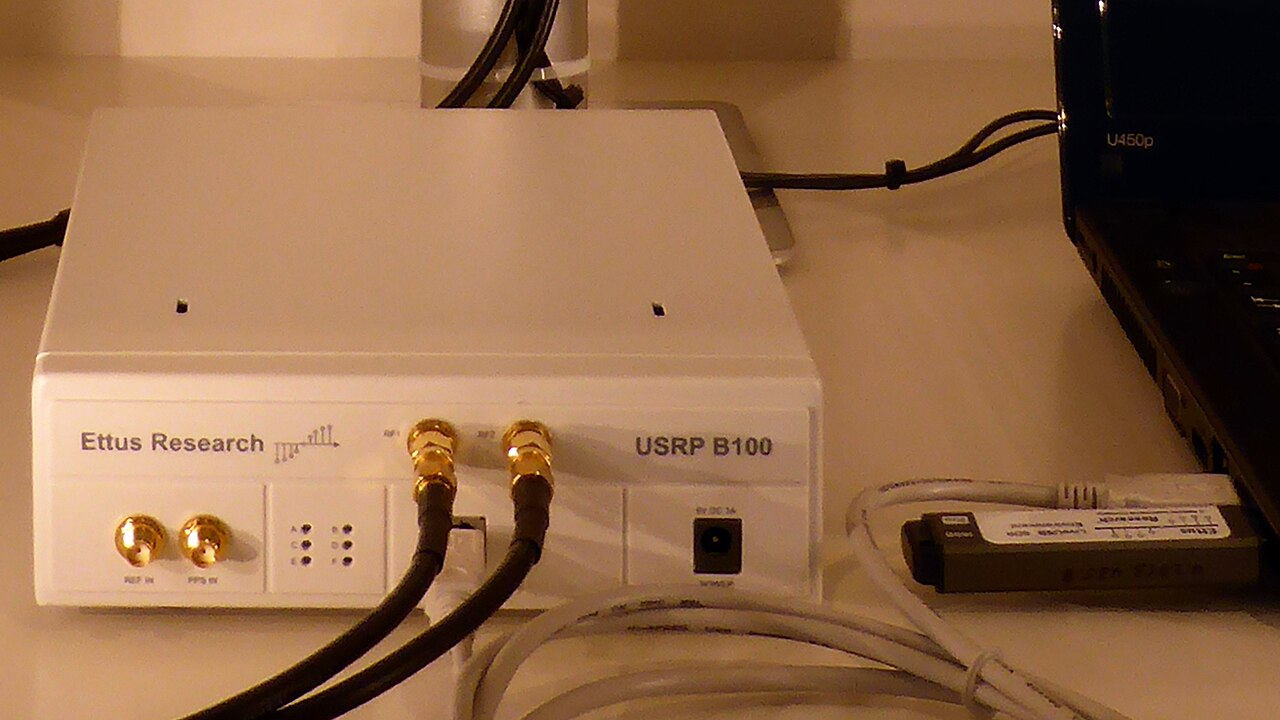
\includegraphics[width=\linewidth]{figure/isac/usrp_b100.jpg}
      \source{https://commons.wikimedia.org/wiki/File:USRP_B100_(crop).jpg}{USRP software-defined radio (illustrative)}
    \column{0.54\textwidth}
      \small
      \begin{itemize}\itemsep4pt
        \item A host PC drives the bench.
        \item An FPGA steers the surface.
        \item USRP plus a converter.
        \item Transmit on the surface.
        \item Receive on a horn antenna.
        \item A target module fakes echoes.
      \end{itemize}
  \end{columns}

  \glossline{RHS = Reconfigurable Holographic Surface \quad
    USRP = Universal Software Radio Peripheral \quad
    FPGA = Field-Programmable Gate Array}

  \vspace{0.2em}
  \takeaway{Two main lobes: one aimed at a user, one at a target.\\One aperture, at the same time.}
\end{frame}

\begin{frame}{Inside the chamber}
  \begin{columns}[T,onlytextwidth]
    \column{0.44\textwidth}
      \centering
      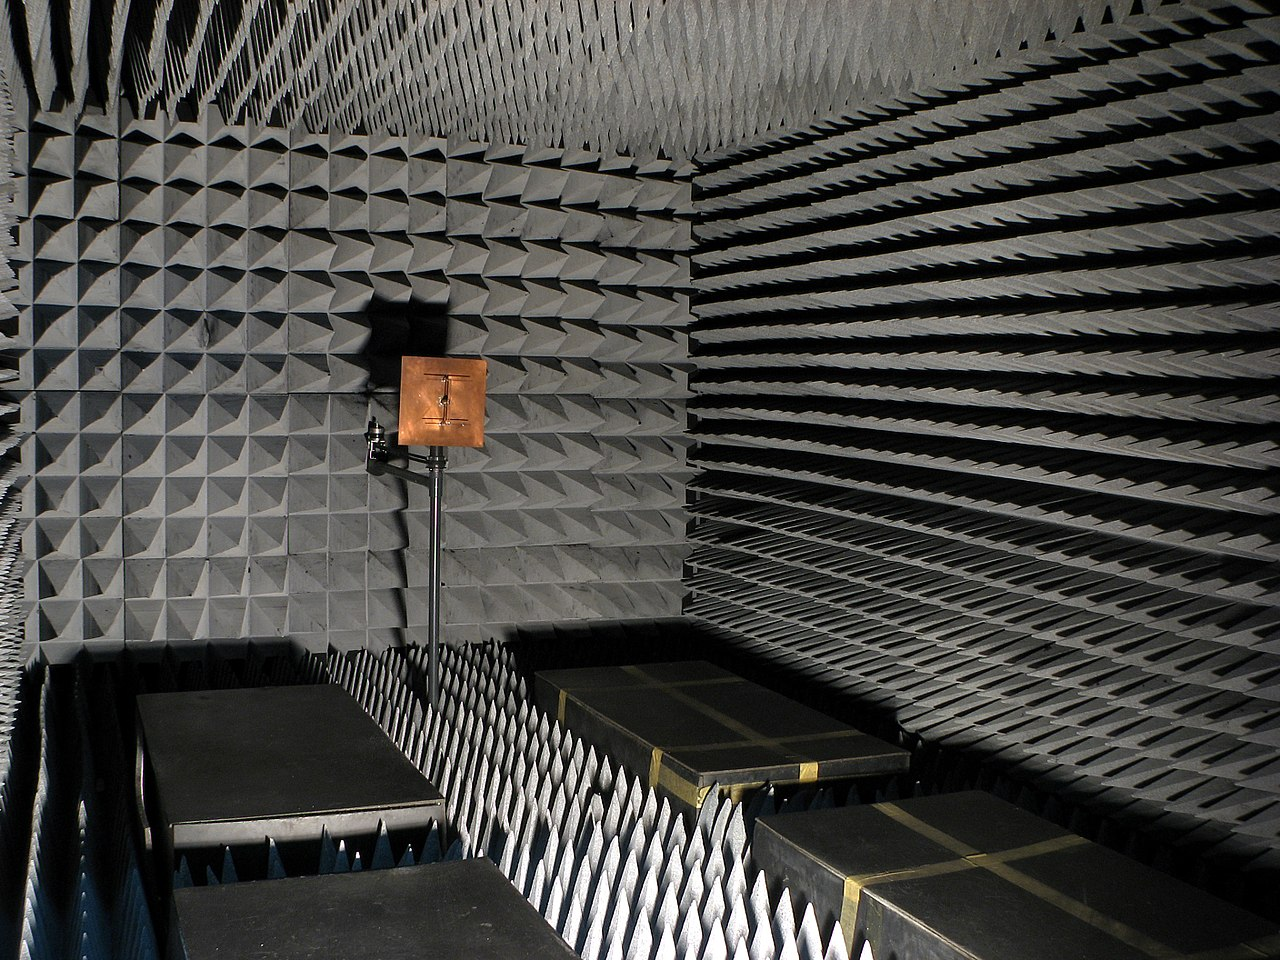
\includegraphics[width=\linewidth]{figure/isac/anechoic_chamber.jpg}
      \source{https://commons.wikimedia.org/wiki/File:Radio-frequency-anechoic-chamber-HDR-0a.jpg}{RF anechoic chamber, Democritus University of Thrace}
    \column{0.52\textwidth}
      \small
      \begin{itemize}\itemsep5pt
        \item Chamber about 4\,m cubed.
        \item Lobe steered to $-50^\circ$, $0^\circ$, $20^\circ$.
        \item Estimated range tracks truth.
        \item Second lobe carries live data.
      \end{itemize}
  \end{columns}

  \vspace{0.3em}
  \qa{Why prove it in an anechoic chamber first?}
     {Because the chamber removes every echo you did not create. If sensing fails
      there, the waveform is wrong; if it fails outdoors, the world is the
      variable.}

  \source{https://ieeexplore.ieee.org/document/10681896}{IEEE/CIC ICCC 2024, Best Demo Award}
\end{frame}

% ACCURACY NOTE: the outdoor and indoor numbers below are the demo's own measured
% accuracies. 15 degrees of angular accuracy is coarse -- that is the honest point of
% the frame. Do not soften it.
\begin{frame}{Measured numbers are humbler}
  \vspace{0.5em}
  \begin{columns}[T,onlytextwidth]
    \column{0.47\textwidth}
      \large\textbf{\textcolor{ranblue}{Range, outdoors}}

      \vspace{0.5em}
      \small
      \begin{itemize}\itemsep4pt
        \item Target: a metal plate
        \item Span: 4--21\,m
        \item Accuracy: about 0.425\,m
      \end{itemize}
    \column{0.47\textwidth}
      \large\textbf{\textcolor{coreorange}{Angle, indoors}}

      \vspace{0.5em}
      \small
      \begin{itemize}\itemsep4pt
        \item Same metal plate
        \item Span: $-60^\circ$ to $+60^\circ$
        \item Accuracy: about $15^\circ$
      \end{itemize}
  \end{columns}

  \vspace{0.9em}
  \ask{Half a metre and fifteen degrees.\\Which applications does that already serve?}
\end{frame}

